\documentclass{standalone}
\usepackage{tikz}
\usetikzlibrary{patterns, positioning}


\begin{document}
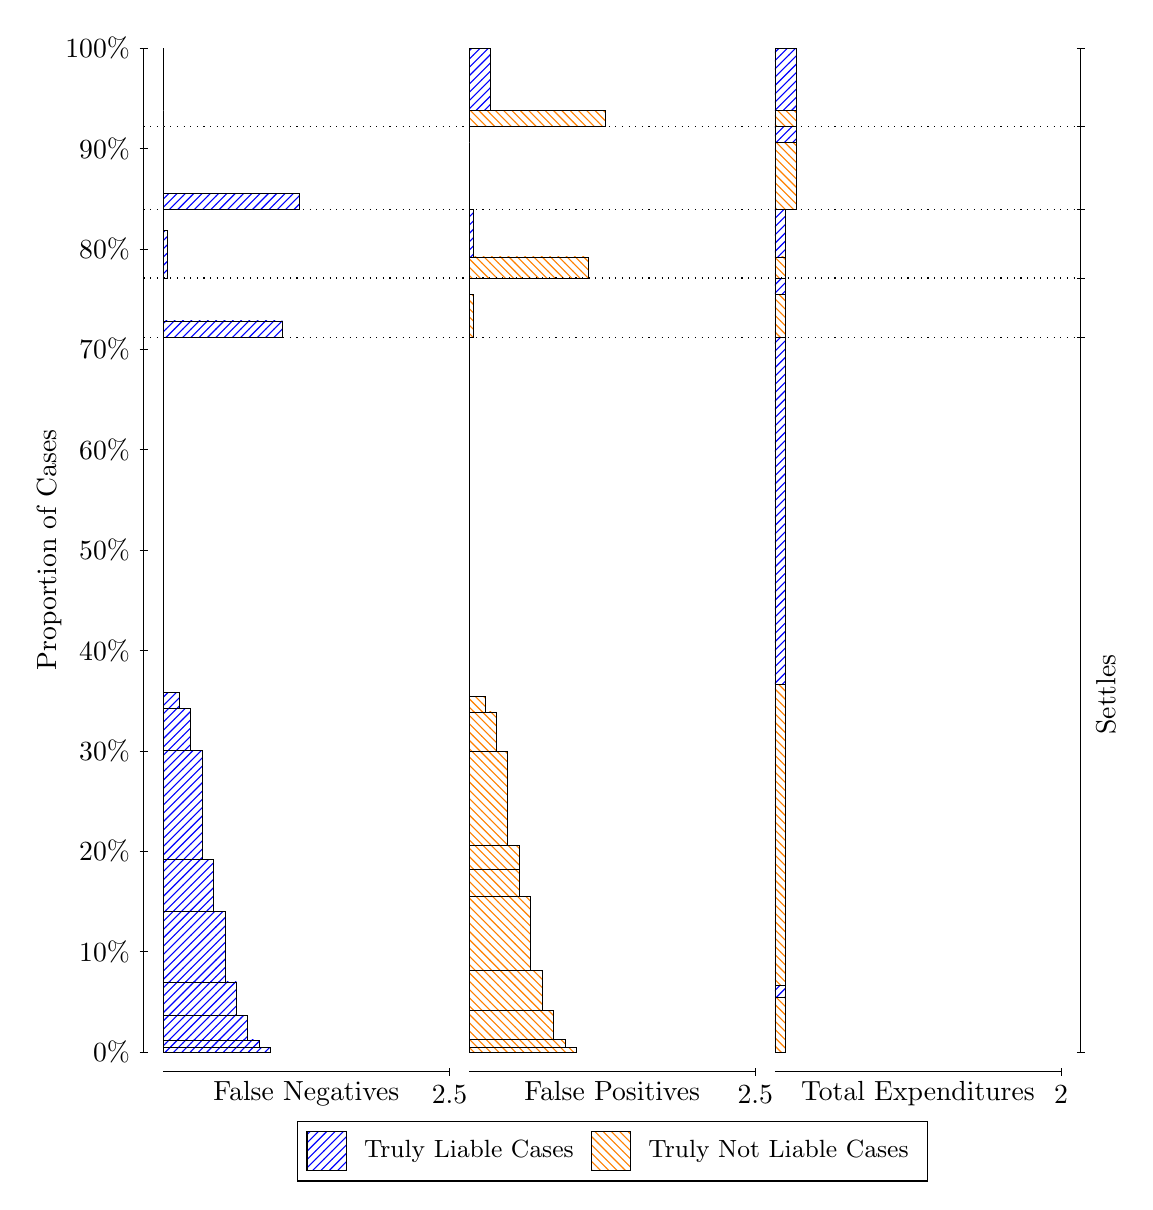
\begin{tikzpicture}
\draw[black, very thin] (1.5,1.75) -- (1.5,14.5);
\node[rotate=90, text=black, anchor=center] at (0.3, 8.125) {Proportion of Cases};
\draw[black, very thin] (1.45,1.75) -- (1.55,1.75);
\node[text=black, anchor=east] at (1.45, 1.75) {0\%};
\draw[black, very thin] (1.45,3.025) -- (1.55,3.025);
\node[text=black, anchor=east] at (1.45, 3.025) {10\%};
\draw[black, very thin] (1.45,4.3) -- (1.55,4.3);
\node[text=black, anchor=east] at (1.45, 4.3) {20\%};
\draw[black, very thin] (1.45,5.575) -- (1.55,5.575);
\node[text=black, anchor=east] at (1.45, 5.575) {30\%};
\draw[black, very thin] (1.45,6.85) -- (1.55,6.85);
\node[text=black, anchor=east] at (1.45, 6.85) {40\%};
\draw[black, very thin] (1.45,8.125) -- (1.55,8.125);
\node[text=black, anchor=east] at (1.45, 8.125) {50\%};
\draw[black, very thin] (1.45,9.4) -- (1.55,9.4);
\node[text=black, anchor=east] at (1.45, 9.4) {60\%};
\draw[black, very thin] (1.45,10.675) -- (1.55,10.675);
\node[text=black, anchor=east] at (1.45, 10.675) {70\%};
\draw[black, very thin] (1.45,11.95) -- (1.55,11.95);
\node[text=black, anchor=east] at (1.45, 11.95) {80\%};
\draw[black, very thin] (1.45,13.225) -- (1.55,13.225);
\node[text=black, anchor=east] at (1.45, 13.225) {90\%};
\draw[black, very thin] (1.45,14.5) -- (1.55,14.5);
\node[text=black, anchor=east] at (1.45, 14.5) {100\%};

\draw[black, very thin] (13.4,1.75) -- (13.4,14.5);
\draw[black, very thin] (13.35,1.75) -- (13.45,1.75);
\node[anchor=west] at (13.35, 1.75) {};
\draw[black, very thin] (13.35,10.828) -- (13.45,10.828);
\node[anchor=west] at (13.35, 10.828) {};
\draw[black, very thin] (13.35,11.579) -- (13.45,11.579);
\node[anchor=west] at (13.35, 11.579) {};
\draw[black, very thin] (13.35,12.45) -- (13.45,12.45);
\node[anchor=west] at (13.35, 12.45) {};
\draw[black, very thin] (13.35,13.502) -- (13.45,13.502);
\node[anchor=west] at (13.35, 13.502) {};
\draw[black, very thin] (13.35,14.5) -- (13.45,14.5);
\node[anchor=west] at (13.35, 14.5) {};

\draw[black, very thin, pattern color=blue, pattern=north east lines] (1.75,1.75) rectangle (3.1125,1.8035);
\draw[black, very thin, pattern color=blue, pattern=north east lines] (1.75,1.8035) rectangle (2.9672,1.9033);
\draw[black, very thin, pattern color=blue, pattern=north east lines] (1.75,1.9033) rectangle (2.8218,2.2122);
\draw[black, very thin, pattern color=blue, pattern=north east lines] (1.75,2.2122) rectangle (2.6765,2.6388);
\draw[black, very thin, pattern color=blue, pattern=north east lines] (1.75,2.6388) rectangle (2.5312,3.5368);
\draw[black, very thin, pattern color=blue, pattern=north east lines] (1.75,3.5368) rectangle (2.3858,4.195);
\draw[black, very thin, pattern color=blue, pattern=north east lines] (1.75,4.195) rectangle (2.2405,5.5845);
\draw[black, very thin, pattern color=blue, pattern=north east lines] (1.75,5.5845) rectangle (2.0952,6.1165);
\draw[black, very thin, pattern color=blue, pattern=north east lines] (1.75,6.1165) rectangle (1.9498,6.3157);
\draw[black, very thin, pattern color=orange, pattern=north west lines] (1.75,6.3157) rectangle (1.75,10.828);
\draw[black, very thin, pattern color=blue, pattern=north east lines] (1.75,10.828) rectangle (3.2578,11.036);
\draw[black, very thin, pattern color=orange, pattern=north west lines] (1.75,11.036) rectangle (1.75,11.579);
\draw[black, very thin, pattern color=blue, pattern=north east lines] (1.75,11.579) rectangle (1.8045,12.182);
\draw[black, very thin, pattern color=orange, pattern=north west lines] (1.75,12.182) rectangle (1.75,12.45);
\draw[black, very thin, pattern color=blue, pattern=north east lines] (1.75,12.45) rectangle (3.4758,12.654);
\draw[black, very thin, pattern color=orange, pattern=north west lines] (1.75,12.654) rectangle (1.75,13.502);
\draw[black, very thin, pattern color=orange, pattern=north west lines] (1.75,13.502) rectangle (1.75,13.705);
\draw[black, very thin, pattern color=blue, pattern=north east lines] (1.75,13.705) rectangle (1.75,14.5);
\draw[black, very thin, pattern color=orange, pattern=north west lines] (5.6333,1.75) rectangle (6.9958,1.8054);
\draw[black, very thin, pattern color=orange, pattern=north west lines] (5.6333,1.8054) rectangle (6.8505,1.9069);
\draw[black, very thin, pattern color=orange, pattern=north west lines] (5.6333,1.9069) rectangle (6.7052,2.2755);
\draw[black, very thin, pattern color=orange, pattern=north west lines] (5.6333,2.2755) rectangle (6.5598,2.7889);
\draw[black, very thin, pattern color=orange, pattern=north west lines] (5.6333,2.7889) rectangle (6.4145,3.7297);
\draw[black, very thin, pattern color=orange, pattern=north west lines] (5.6333,3.7297) rectangle (6.2692,4.064);
\draw[black, very thin, pattern color=orange, pattern=north west lines] (5.6333,4.064) rectangle (6.2692,4.3742);
\draw[black, very thin, pattern color=orange, pattern=north west lines] (5.6333,4.3742) rectangle (6.1238,5.5693);
\draw[black, very thin, pattern color=orange, pattern=north west lines] (5.6333,5.5693) rectangle (5.9785,6.0694);
\draw[black, very thin, pattern color=orange, pattern=north west lines] (5.6333,6.0694) rectangle (5.8332,6.2628);
\draw[black, very thin, pattern color=blue, pattern=north east lines] (5.6333,6.2628) rectangle (5.6333,10.828);
\draw[black, very thin, pattern color=orange, pattern=north west lines] (5.6333,10.828) rectangle (5.6878,11.372);
\draw[black, very thin, pattern color=blue, pattern=north east lines] (5.6333,11.372) rectangle (5.6333,11.579);
\draw[black, very thin, pattern color=orange, pattern=north west lines] (5.6333,11.579) rectangle (7.1412,11.847);
\draw[black, very thin, pattern color=blue, pattern=north east lines] (5.6333,11.847) rectangle (5.6878,12.45);
\draw[black, very thin, pattern color=orange, pattern=north west lines] (5.6333,12.45) rectangle (5.6333,13.298);
\draw[black, very thin, pattern color=blue, pattern=north east lines] (5.6333,13.298) rectangle (5.6333,13.502);
\draw[black, very thin, pattern color=orange, pattern=north west lines] (5.6333,13.502) rectangle (7.3592,13.705);
\draw[black, very thin, pattern color=blue, pattern=north east lines] (5.6333,13.705) rectangle (5.9058,14.5);
\draw[black, very thin, pattern color=orange, pattern=north west lines] (9.5167,1.75) rectangle (9.6529,2.4435);
\draw[black, very thin, pattern color=blue, pattern=north east lines] (9.5167,2.4435) rectangle (9.6529,2.5967);
\draw[black, very thin, pattern color=orange, pattern=north west lines] (9.5167,2.5967) rectangle (9.6529,6.416);
\draw[black, very thin, pattern color=blue, pattern=north east lines] (9.5167,6.416) rectangle (9.6529,10.828);
\draw[black, very thin, pattern color=orange, pattern=north west lines] (9.5167,10.828) rectangle (9.6529,11.372);
\draw[black, very thin, pattern color=blue, pattern=north east lines] (9.5167,11.372) rectangle (9.6529,11.579);
\draw[black, very thin, pattern color=orange, pattern=north west lines] (9.5167,11.579) rectangle (9.6529,11.847);
\draw[black, very thin, pattern color=blue, pattern=north east lines] (9.5167,11.847) rectangle (9.6529,12.45);
\draw[black, very thin, pattern color=orange, pattern=north west lines] (9.5167,12.45) rectangle (9.7892,13.298);
\draw[black, very thin, pattern color=blue, pattern=north east lines] (9.5167,13.298) rectangle (9.7892,13.502);
\draw[black, very thin, pattern color=orange, pattern=north west lines] (9.5167,13.502) rectangle (9.7892,13.705);
\draw[black, very thin, pattern color=blue, pattern=north east lines] (9.5167,13.705) rectangle (9.7892,14.5);
\draw[black, dotted] (1.5,10.828) -- (13.4,10.828);
\draw[black, dotted] (1.5,11.579) -- (13.4,11.579);
\draw[black, dotted] (1.5,12.45) -- (13.4,12.45);
\draw[black, dotted] (1.5,13.502) -- (13.4,13.502);
\draw[black, very thin] (1.75,1.5) -- (5.3833,1.5);
\node[text=black, anchor=north] at (3.5667, 1.5) {False Negatives};
\draw[black, very thin] (5.3833,1.45) -- (5.3833,1.55);
\node[text=black, anchor=north] at (5.3833, 1.45) {2.5};

\draw[black, very thin] (5.6333,1.5) -- (9.2667,1.5);
\node[text=black, anchor=north] at (7.45, 1.5) {False Positives};
\draw[black, very thin] (9.2667,1.45) -- (9.2667,1.55);
\node[text=black, anchor=north] at (9.2667, 1.45) {2.5};

\draw[black, very thin] (9.5167,1.5) -- (13.15,1.5);
\node[text=black, anchor=north] at (11.333, 1.5) {Total Expenditures};
\draw[black, very thin] (13.15,1.45) -- (13.15,1.55);
\node[text=black, anchor=north] at (13.15, 1.45) {2};

\node[text=black, centered, rotate=90] at (13.72, 6.2892) {Settles};





\draw (7.449999999999999,1.5) node[draw=none] (baseCoordinate) {};
\begin{scope}[align=center]
        \matrix[scale=0.5, draw=black, below=0.5cm of baseCoordinate, nodes={draw}, column sep=0.1cm]{
            \node[rectangle, draw, minimum width=0.5cm, minimum height=0.5cm, pattern color=blue, pattern=north east lines] {}; &
            \node[draw=none, font=\small, text=black] (B) {Truly Liable Cases}; &
            \node[rectangle, draw, minimum width=0.5cm, minimum height=0.5cm, pattern color=orange, pattern=north west lines] {}; &
            \node[draw=none, font=\small, text=black] (B) {Truly Not Liable Cases}; \\
            };
\end{scope}

\end{tikzpicture}
\end{document}